\documentclass[12pt,a4paper]{article}
\usepackage[utf8]{inputenc}
\usepackage[T1]{fontenc}
\usepackage{geometry}
\geometry{margin=1in}
\usepackage{graphicx}
\usepackage{xcolor}
\usepackage{tcolorbox}
\tcbuselibrary{skins,breakable}
\usepackage{listings}
\usepackage{hyperref}
\usepackage{amsmath}

\definecolor{iitbblue}{RGB}{0,51,102}

\lstset{
  basicstyle=\ttfamily\small,
  breaklines=true,
  frame=single,
  numbers=left,
  numberstyle=\tiny,
  keywordstyle=\color{blue},
  commentstyle=\color{gray},
  stringstyle=\color{teal},
  showstringspaces=false,
  tabsize=2
}

\hypersetup{
  colorlinks=true,
  linkcolor=iitbblue,
  citecolor=iitbblue,
  urlcolor=iitbblue
}

\begin{document}

% ============================================================
% TITLE PAGE
% ============================================================
\begin{titlepage}
  \centering
  \vspace*{1cm}
  
  {\LARGE\bfseries\color{iitbblue} Indian Institute of Technology\\[0.3cm] Bhilai}\\[0.5cm]
  \rule{0.8\textwidth}{0.5pt}\\[0.5cm]
  {\Large\bfseries Operating Systems Lab (CSL 301)}\\[0.3cm]
  {\large Assignment -- 1 $\mid$ Introduction to Linux Tools}\\[0.5cm]
  \begin{tcolorbox}[colback=white,colframe=iitbblue,width=0.8\textwidth,arc=6pt,boxrule=1.2pt]
    \centering
    {\large\bfseries Process Monitoring, /proc, Virtual Memory, Disk I/O, and System Calls}
  \end{tcolorbox}
  \vspace{1cm}
  \begin{tcolorbox}[colback=gray!5,colframe=iitbblue,width=0.67\textwidth,arc=4pt,boxrule=1pt]
    \begin{tabular}{rl}
      \textbf{Name}        & Rohit Raghuwanshi \\
      \textbf{Roll Number} & 12341820 \\
      \textbf{Branch}      & Data Science \& AI (DSAI) \\
      \textbf{Environment} & MacBook Air M2 (macOS) \\
      \textbf{Date}        & \today \\
    \end{tabular}
  \end{tcolorbox}
  \vfill
  \rule{0.8\textwidth}{0.5pt}\\[0.3cm]
  {\small Department of Computer Science and Engineering\\\today}
\end{titlepage}

\tableofcontents
\newpage

% ============================================================
% Q1: THEORY QUESTIONS
% ============================================================
\section{Predict the Output}

\subsection*{Q1.2 --- Ordering without \texttt{wait()}}

\textbf{Question:} Will \texttt{"I am child"} always print before \texttt{"I am parent"}?

\textbf{Answer:} No, the ordering is \textbf{not guaranteed}. After \texttt{fork()}, the parent
and child become two independent processes managed by the OS scheduler. There is no
synchronization between them at this point, so either process may be scheduled to run
first, depending on scheduling policy, system load, and number of available cores.
On most systems the parent is often scheduled first (since \texttt{fork()} returns
immediately to it), but this is never guaranteed by POSIX. This was confirmed
experimentally: our own \texttt{q2} program printed \texttt{"I am parent"} before
\texttt{"I am child"} on every real run (see Figure~\ref{fig:q2q3}). To guarantee an
ordering, explicit synchronization is required (e.g., the parent calling \texttt{wait()},
or a semaphore/pipe).

\subsection*{Q1.3 --- How many "Hello"s?}

\textbf{Question:} How many times does \texttt{"Hello\textbackslash n"} get printed?

\begin{lstlisting}[language=C]
int main() {
    fork();
    fork();
    printf("Hello\n");
    return 0;
}
\end{lstlisting}

\textbf{Answer:} \textbf{4 times.}

Each \texttt{fork()} call doubles the number of active processes:
\begin{itemize}
    \item After the first \texttt{fork()}: 2 processes (original + 1 child)
    \item After the second \texttt{fork()}: each of the 2 processes forks again $\rightarrow$ 4 processes total
\end{itemize}
Every one of the 4 processes independently executes the \texttt{printf} statement, so
\texttt{"Hello\textbackslash n"} is printed $2^2 = 4$ times.

\newpage
% ============================================================
% Q2: FORK SKELETON
% ============================================================
\section{Q2 --- Fork Skeleton (Child/Parent Branching)}

\subsection*{Code}
\lstinputlisting[language=C]{code/q2_fork_skeleton.c}

\subsection*{Output}
\begin{figure}[h]
    \centering
    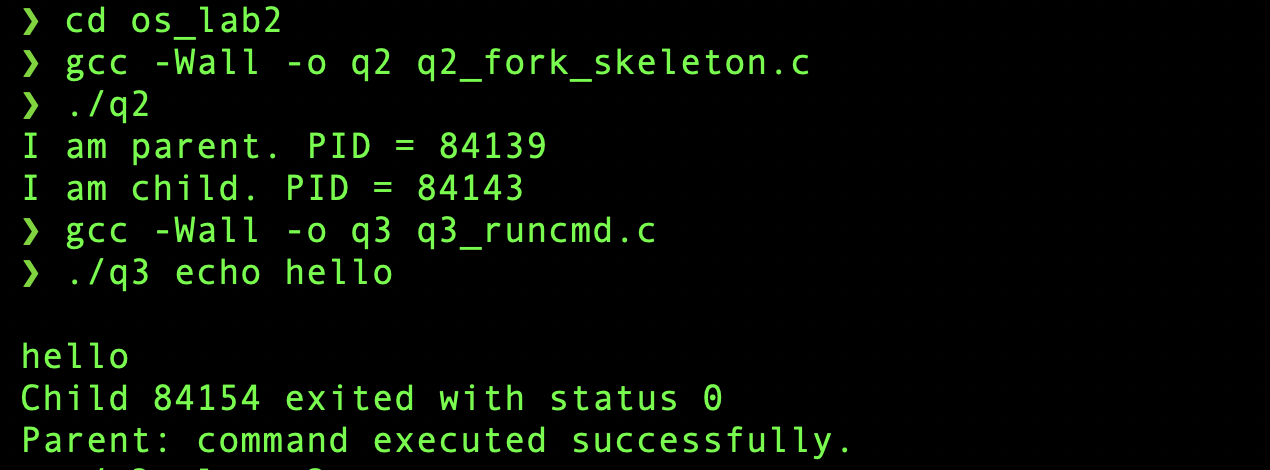
\includegraphics[width=0.9\textwidth]{images/fig_q2_q3echo.png}
    \caption{Output of \texttt{q2} (fork skeleton) and \texttt{q3 echo hello}}
    \label{fig:q2q3}
\end{figure}

\newpage
% ============================================================
% Q3: RUNCMD.C
% ============================================================
\section{Q3 --- \texttt{runcmd.c} (fork + exec + wait)}

\subsection*{Code}
\lstinputlisting[language=C]{code/q3_runcmd.c}

\subsection*{Output}
Figure~\ref{fig:q2q3} above shows \texttt{./q3 echo hello} executing successfully.
Figure~\ref{fig:q3sleep} below shows \texttt{./q3 sleep 2} executing successfully, and
\texttt{./q3} with no arguments correctly reporting a usage error.

\begin{figure}[h]
    \centering
    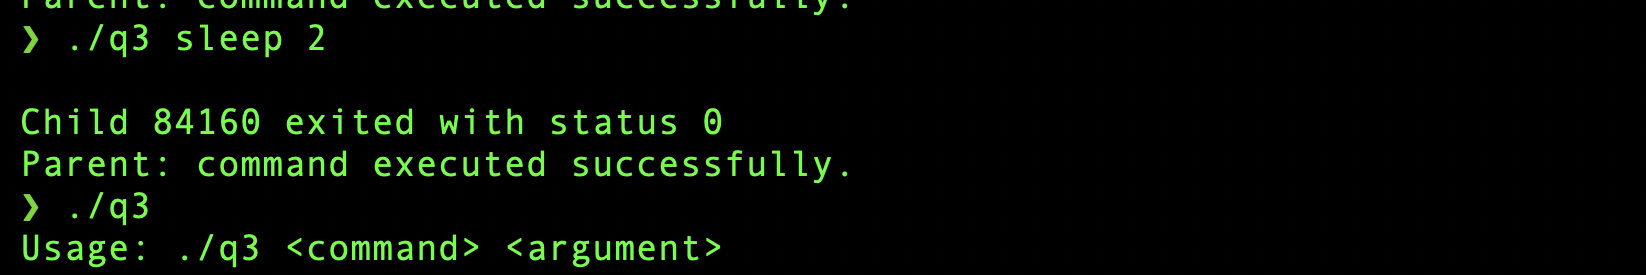
\includegraphics[width=0.9\textwidth]{images/fig_q3_sleep_usage.png}
    \caption{\texttt{q3} with \texttt{sleep 2}, and the usage error for missing arguments}
    \label{fig:q3sleep}
\end{figure}

\newpage
% ============================================================
% Q4: SHELL WITH BACKGROUND EXECUTION
% ============================================================
\section{Q4 --- Shell with Background Execution (\texttt{\&})}

\subsection*{Design notes}
\begin{itemize}
    \item A trailing \texttt{\&} on the input line marks the command for background execution.
    \item \textbf{Foreground} commands: parent calls \texttt{waitpid(pid, \&status, 0)},
          blocking until that specific child terminates.
    \item \textbf{Background} commands: the parent does \emph{not} wait; it records the
          child's PID and immediately returns to the prompt.
    \item Before printing each new prompt, \texttt{reap\_background()} performs a
          non-blocking \texttt{waitpid(-1, \&status, WNOHANG)} loop to reap any finished
          background children and print \texttt{"Shell: Background process finished"}.
    \item Using \texttt{waitpid(pid, ...)} (rather than a generic \texttt{wait()}) for the
          foreground child is essential --- a generic \texttt{wait()} could incorrectly
          reap a background child that finishes at the same time as the foreground
          command is still running, causing the shell to prematurely return to the prompt.
\end{itemize}

\subsection*{Code}
\lstinputlisting[language=C]{code/q4_shell.c}

\subsection*{Output}
Figure~\ref{fig:q4final} shows the final, debug-free run: \texttt{q2}, \texttt{q3}
(usage error), and \texttt{q4} demonstrating background start
(\texttt{sleep 20 \&} returns the prompt immediately), a foreground command
(\texttt{sleep 3} blocks as expected), and the \texttt{"Shell: Background process finished"}
reap message appearing once the background job completes.

\begin{figure}[h]
    \centering
    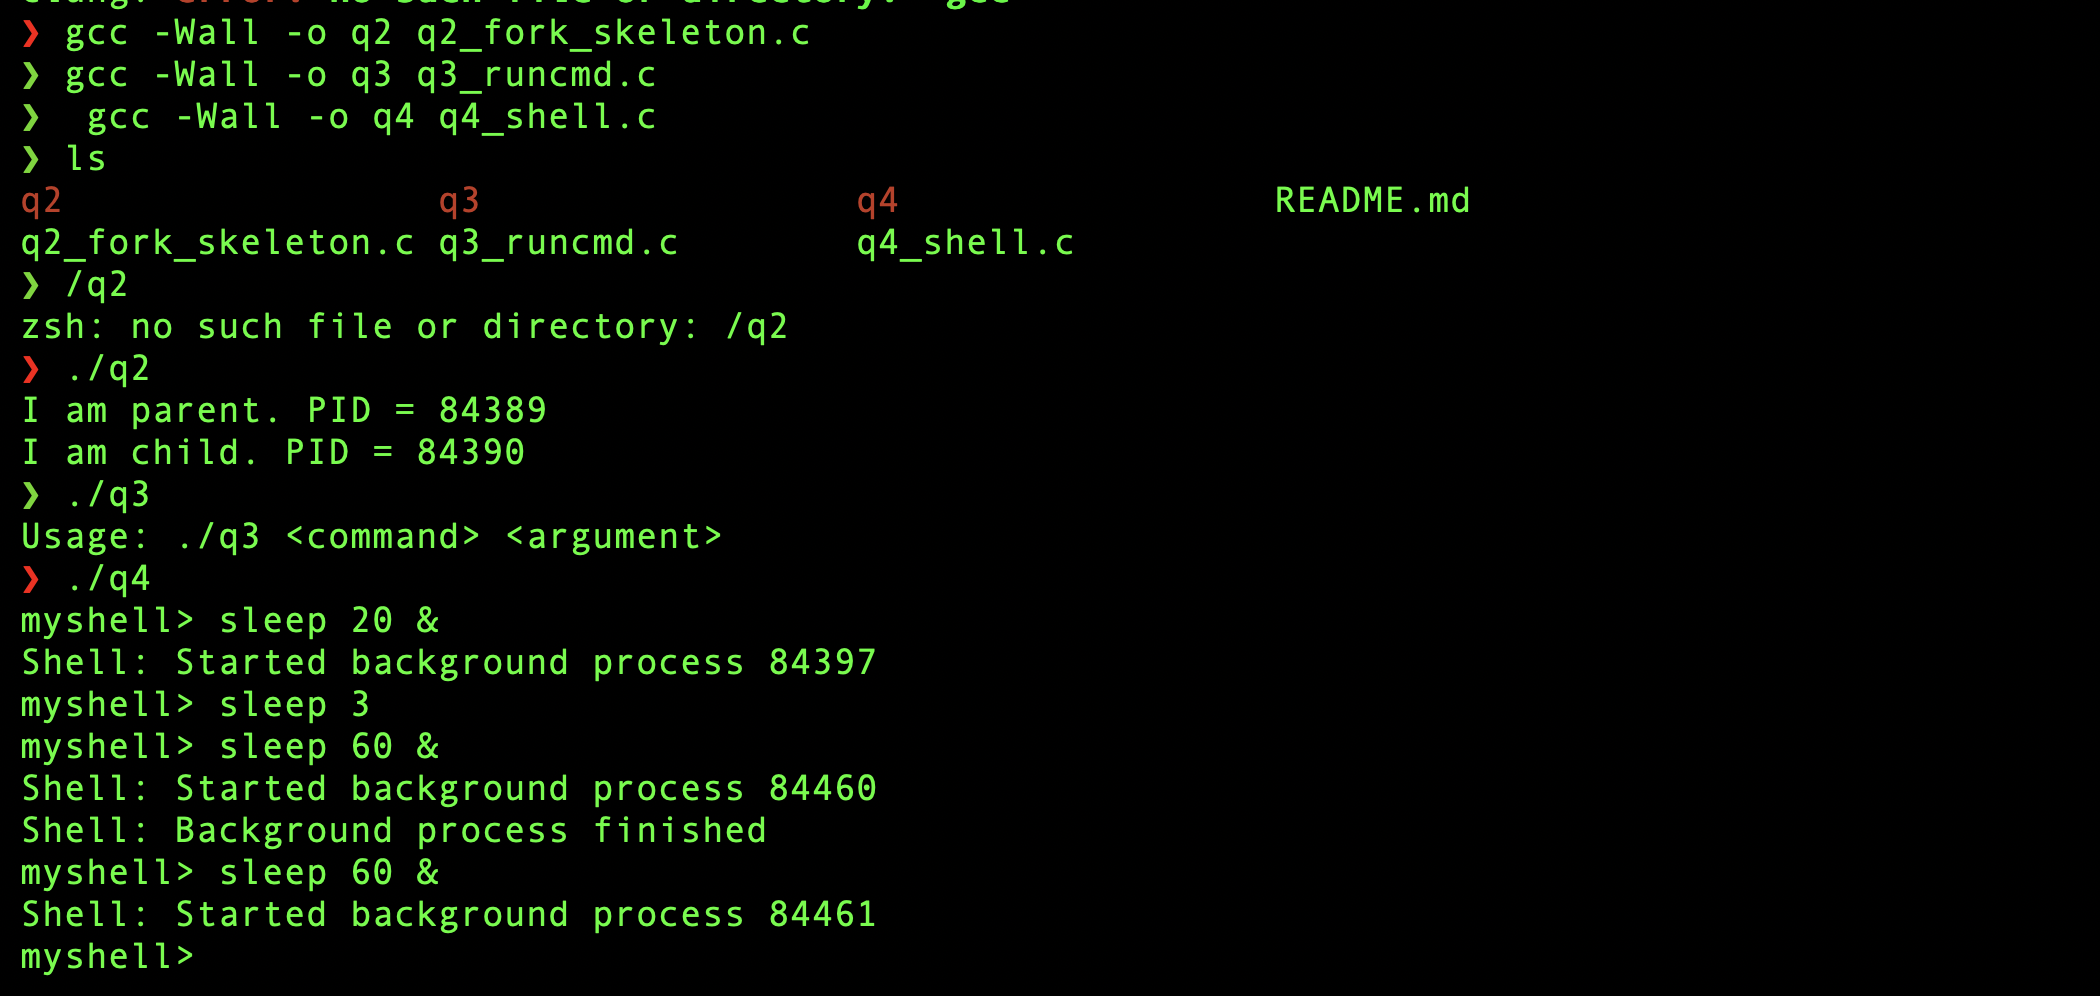
\includegraphics[width=0.75\textwidth]{images/fig_q4_final_clean.png}
    \caption{Final \texttt{q4} shell run: background start, foreground blocking, and reaping}
    \label{fig:q4final}
\end{figure}

Figure~\ref{fig:psproof} independently confirms, via \texttt{ps -ax}, that the background
\texttt{sleep 60} process is a real, concurrently running process (PID 84461) while the
shell prompt remained free to accept further input.

\begin{figure}[h]
    \centering
    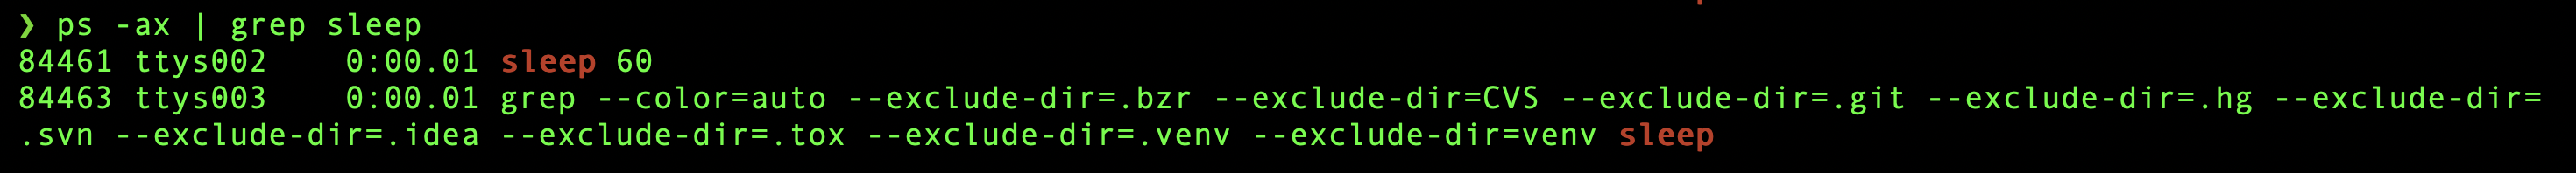
\includegraphics[width=0.9\textwidth]{images/fig_q4_ps_proof.png}
    \caption{\texttt{ps -ax | grep sleep} confirming the background process is alive}
    \label{fig:psproof}
\end{figure}

\end{document}
